\begin{section}{IV-replacement (stateless) attack}
\label{sec:iv_replacement_stateless}

\begin{figure}[!ht]
	\centering
	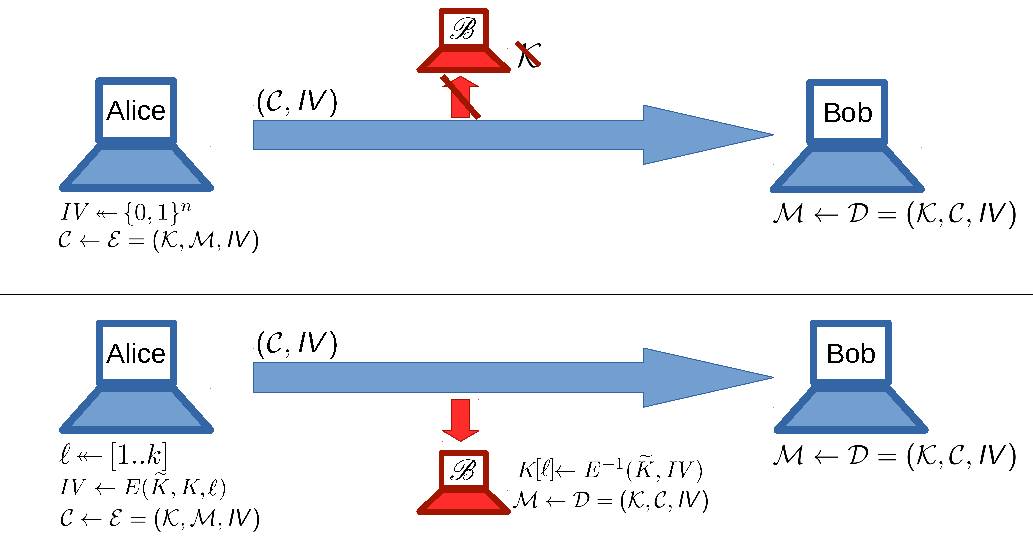
\includegraphics[width=\textwidth]{image/iv_replacement_stateless}
	\caption{IV replacement (stateless) attack.}
	\label{fig:iv_replacement_stateless}
\end{figure}

\begin{subsection}{Grundidee}

Der zweite Ansatz für eine ASA ist ebenfalls die IV replacement attack, diesmal für ein symmetrisches stateless Schema $\Pi = (\mathcal{E}, \mathcal{D}, \mathcal{K})$. Ansatzpunkt bei diesem Angriff ist wieder die Generierung des nonce. Grundgedanke ist es, bitweise und mit einer gewissen zufälligen Verteilung Teile von $\mathcal{K}$ im IV zu versteckt. Bei jeder Generierung des IV wird ein zufälliges Bit von $\mathcal{K}$ im IV versteckt. Der Schlüssel $\mathcal{K}$ kann so nach endlicher Zeit von $\mathscr{B}$ bitweise und über mehrere Übertragungen hinweg rekonstruiert werden.

\end{subsection}

\begin{subsection}{Durchführung}

Alice geniert sich mit einer Subversion der Funktion $E$, in der der Masterschlüssel $\widetilde{\mathcal{K}}$ verwendet wird, einen IV. Dieser ist allerdings nicht ganz zufällig. Er ist so geschickt gewählt, dass er ein zufälliges Bit $\ell$ des geheimen Schlüssels $\mathcal{K}$ enthält. Dieser IV geht wie beim regulären $\Pi$ in die Verschlüsselungsfunktion $\mathcal{E}$ ein. Big Brother ist nun in der Lage mit dem Masterschlüssel $\widetilde{\mathcal{K}}$ und der Umkehrfunktion $E^{-1}$ von $E$ ein Bit $\ell$ von $\mathcal{K}$ zu berechnen.

\end{subsection}

\begin{subsection}{Entdeckbarkeit}

Eine solche Subversion ist noch schwerer entdeckbar als die vorherige Angriffstechnik. Selbst ein Reset des Systems kann nicht zum Entdecken der Subversion führen. Je mehr Bits von $\mathcal{K}$ in einer Übertragung verraten werden, desto höher ist die Wahrscheinlichkeit, dass die Subversion entdeckt wird.

\end{subsection}

\end{section}